

\tikzset{every picture/.style={line width=0.75pt}} %set default line width to 0.75pt        

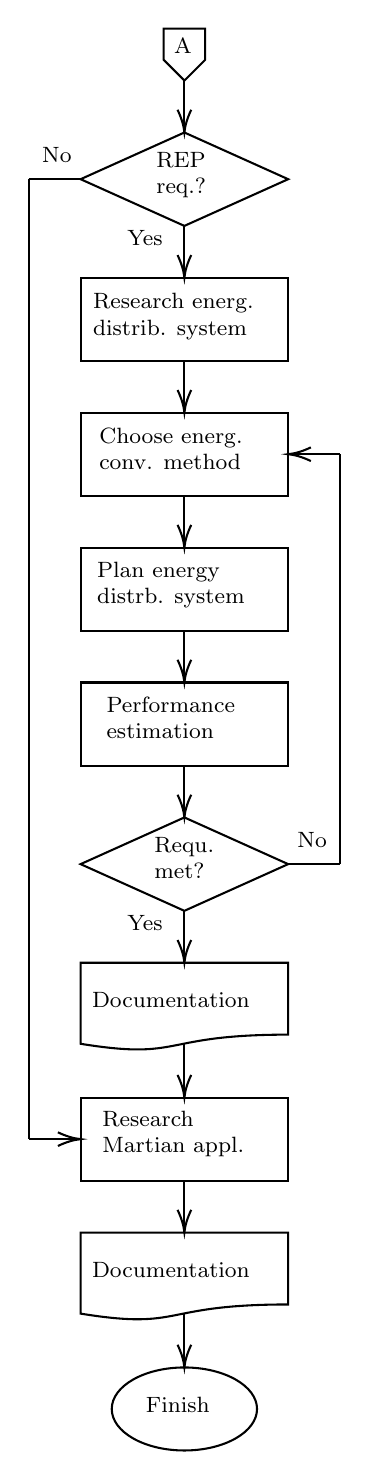
\begin{tikzpicture}[x=0.75pt,y=0.75pt,yscale=-1,xscale=1]
%uncomment if require: \path (0,882); %set diagram left start at 0, and has height of 882

%Pentagon Arrow [id:dp6295335837224703] 
\draw   (365,45) -- (365,60) -- (355,70) -- (345,60) -- (345,45) -- cycle ;

%Shape: Rectangle [id:dp9114846783986272] 
\draw   (305,165) -- (405,165) -- (405,205) -- (305,205) -- cycle ;

%Straight Lines [id:da1841951473424126] 
\draw    (355,70) -- (355,93) ;
\draw [shift={(355,95)}, rotate = 270] [color={rgb, 255:red, 0; green, 0; blue, 0 }  ][line width=0.75]    (10.93,-3.29) .. controls (6.95,-1.4) and (3.31,-0.3) .. (0,0) .. controls (3.31,0.3) and (6.95,1.4) .. (10.93,3.29)   ;
%Shape: Diamond [id:dp3275955259803509] 
\draw   (355,95) -- (405,117.5) -- (355,140) -- (305,117.5) -- cycle ;
%Straight Lines [id:da6311173750553984] 
\draw    (355,140) -- (355,163) ;
\draw [shift={(355,165)}, rotate = 270] [color={rgb, 255:red, 0; green, 0; blue, 0 }  ][line width=0.75]    (10.93,-3.29) .. controls (6.95,-1.4) and (3.31,-0.3) .. (0,0) .. controls (3.31,0.3) and (6.95,1.4) .. (10.93,3.29)   ;

%Shape: Rectangle [id:dp913835377980921] 
\draw   (305,230) -- (405,230) -- (405,270) -- (305,270) -- cycle ;

%Straight Lines [id:da3649991025923325] 
\draw    (355,205) -- (355,228) ;
\draw [shift={(355,230)}, rotate = 270] [color={rgb, 255:red, 0; green, 0; blue, 0 }  ][line width=0.75]    (10.93,-3.29) .. controls (6.95,-1.4) and (3.31,-0.3) .. (0,0) .. controls (3.31,0.3) and (6.95,1.4) .. (10.93,3.29)   ;
%Straight Lines [id:da43992652550284816] 
\draw    (355,270) -- (355,293) ;
\draw [shift={(355,295)}, rotate = 270] [color={rgb, 255:red, 0; green, 0; blue, 0 }  ][line width=0.75]    (10.93,-3.29) .. controls (6.95,-1.4) and (3.31,-0.3) .. (0,0) .. controls (3.31,0.3) and (6.95,1.4) .. (10.93,3.29)   ;
%Shape: Rectangle [id:dp9403171441896898] 
\draw   (305,295) -- (405,295) -- (405,335) -- (305,335) -- cycle ;

%Shape: Rectangle [id:dp553852729933479] 
\draw   (305,360) -- (405,360) -- (405,400) -- (305,400) -- cycle ;
%Straight Lines [id:da1550632508471741] 
\draw    (355,335) -- (355,358) ;
\draw [shift={(355,360)}, rotate = 270] [color={rgb, 255:red, 0; green, 0; blue, 0 }  ][line width=0.75]    (10.93,-3.29) .. controls (6.95,-1.4) and (3.31,-0.3) .. (0,0) .. controls (3.31,0.3) and (6.95,1.4) .. (10.93,3.29)   ;
%Straight Lines [id:da1341632742496266] 
\draw    (355,400) -- (355,423) ;
\draw [shift={(355,425)}, rotate = 270] [color={rgb, 255:red, 0; green, 0; blue, 0 }  ][line width=0.75]    (10.93,-3.29) .. controls (6.95,-1.4) and (3.31,-0.3) .. (0,0) .. controls (3.31,0.3) and (6.95,1.4) .. (10.93,3.29)   ;
%Shape: Diamond [id:dp8080302672223327] 
\draw   (355,425) -- (405,447.5) -- (355,470) -- (305,447.5) -- cycle ;

%Straight Lines [id:da3135121459732009] 
\draw    (407,250) -- (430,250) ;
\draw [shift={(405,250)}, rotate = 0] [color={rgb, 255:red, 0; green, 0; blue, 0 }  ][line width=0.75]    (10.93,-3.29) .. controls (6.95,-1.4) and (3.31,-0.3) .. (0,0) .. controls (3.31,0.3) and (6.95,1.4) .. (10.93,3.29)   ;
%Straight Lines [id:da1661173997317298] 
\draw    (430,250) -- (430,447.5) ;
%Straight Lines [id:da013009727986448727] 
\draw    (430,447.5) -- (405,447.5) ;

%Straight Lines [id:da8133901261188266] 
\draw    (355,470) -- (355,493) ;
\draw [shift={(355,495)}, rotate = 270] [color={rgb, 255:red, 0; green, 0; blue, 0 }  ][line width=0.75]    (10.93,-3.29) .. controls (6.95,-1.4) and (3.31,-0.3) .. (0,0) .. controls (3.31,0.3) and (6.95,1.4) .. (10.93,3.29)   ;

%Flowchart: Document [id:dp6420835715080364] 
\draw   (305,495) -- (405,495) -- (405,529.65) .. controls (342.5,529.65) and (355,542.15) .. (305,534.06) -- cycle ;

%Straight Lines [id:da3287541689868827] 
\draw    (355,534) -- (355,558) ;
\draw [shift={(355,560)}, rotate = 270] [color={rgb, 255:red, 0; green, 0; blue, 0 }  ][line width=0.75]    (10.93,-3.29) .. controls (6.95,-1.4) and (3.31,-0.3) .. (0,0) .. controls (3.31,0.3) and (6.95,1.4) .. (10.93,3.29)   ;

%Shape: Rectangle [id:dp9760404082725573] 
\draw   (305,560) -- (405,560) -- (405,600) -- (305,600) -- cycle ;
%Flowchart: Document [id:dp2517134736579656] 
\draw   (305,625) -- (405,625) -- (405,659.65) .. controls (342.5,659.65) and (355,672.15) .. (305,664.06) -- cycle ;

%Straight Lines [id:da5089558784451147] 
\draw    (355,664) -- (355,688) ;
\draw [shift={(355,690)}, rotate = 270] [color={rgb, 255:red, 0; green, 0; blue, 0 }  ][line width=0.75]    (10.93,-3.29) .. controls (6.95,-1.4) and (3.31,-0.3) .. (0,0) .. controls (3.31,0.3) and (6.95,1.4) .. (10.93,3.29)   ;

%Straight Lines [id:da19223774212748634] 
\draw    (355,600) -- (355,623) ;
\draw [shift={(355,625)}, rotate = 270] [color={rgb, 255:red, 0; green, 0; blue, 0 }  ][line width=0.75]    (10.93,-3.29) .. controls (6.95,-1.4) and (3.31,-0.3) .. (0,0) .. controls (3.31,0.3) and (6.95,1.4) .. (10.93,3.29)   ;
%Straight Lines [id:da9396270466808674] 
\draw    (280,580) -- (303,580) ;
\draw [shift={(305,580)}, rotate = 180] [color={rgb, 255:red, 0; green, 0; blue, 0 }  ][line width=0.75]    (10.93,-3.29) .. controls (6.95,-1.4) and (3.31,-0.3) .. (0,0) .. controls (3.31,0.3) and (6.95,1.4) .. (10.93,3.29)   ;
%Straight Lines [id:da020572157364605825] 
\draw    (280,117.5) -- (305,117.5) ;

%Straight Lines [id:da680181864059918] 
\draw    (280,117.5) -- (280,580) ;
%Shape: Ellipse [id:dp16223416818247482] 
\draw   (320,710) .. controls (320,698.95) and (335.67,690) .. (355,690) .. controls (374.33,690) and (390,698.95) .. (390,710) .. controls (390,721.05) and (374.33,730) .. (355,730) .. controls (335.67,730) and (320,721.05) .. (320,710) -- cycle ;

% Text Node
\draw (348.5,48) node [anchor=north west][inner sep=0.75pt]  [font=\footnotesize] [align=left] {A};
% Text Node
\draw (309.5,171) node [anchor=north west][inner sep=0.75pt]  [font=\footnotesize] [align=left] {Research energ.\\distrib. system};
% Text Node
\draw (340,103) node [anchor=north west][inner sep=0.75pt]  [font=\footnotesize] [align=left] {REP\\req.?};
% Text Node
\draw (326,140.5) node [anchor=north west][inner sep=0.75pt]  [font=\footnotesize] [align=left] {Yes};
% Text Node
\draw (312.5,236) node [anchor=north west][inner sep=0.75pt]  [font=\footnotesize] [align=left] {Choose energ.\\conv. method};
% Text Node
\draw (311.5,300.5) node [anchor=north west][inner sep=0.75pt]  [font=\footnotesize] [align=left] {Plan energy\\distrb. system};
% Text Node
\draw (316,365.5) node [anchor=north west][inner sep=0.75pt]  [font=\footnotesize] [align=left] {Performance\\estimation};
% Text Node
\draw (339,433) node [anchor=north west][inner sep=0.75pt]  [font=\footnotesize] [align=left] {Requ.\\met?};
% Text Node
\draw (408,430.5) node [anchor=north west][inner sep=0.75pt]  [font=\footnotesize] [align=left] {No};
% Text Node
\draw (326,470.5) node [anchor=north west][inner sep=0.75pt]  [font=\footnotesize] [align=left] {Yes};
% Text Node
\draw (309,508) node [anchor=north west][inner sep=0.75pt]  [font=\footnotesize] [align=left] {Documentation};
% Text Node
\draw (314,565) node [anchor=north west][inner sep=0.75pt]  [font=\footnotesize] [align=left] {Research\\Martian appl.};
% Text Node
\draw (309,638) node [anchor=north west][inner sep=0.75pt]  [font=\footnotesize] [align=left] {Documentation};
% Text Node
\draw (285,100.5) node [anchor=north west][inner sep=0.75pt]  [font=\footnotesize] [align=left] {No};
% Text Node
\draw (335,703) node [anchor=north west][inner sep=0.75pt]  [font=\footnotesize] [align=left] {Finish};


\end{tikzpicture}
